\documentclass{standalone}

\usepackage{libertinus}
\usepackage[T1]{fontenc}
\renewcommand*\familydefault{\sfdefault}

\usepackage{DejaVuSansMono}

\usepackage{tikz}
\usetikzlibrary{decorations.pathmorphing, decorations.pathreplacing, decorations.shapes}
\tikzset{every path/.style={semithick}}

\newcommand{\queuesx}[2]{
  \draw (#1+0.25,#2+0.35) -- ++(0,0.8);
  \draw (#1+0.75,#2+0.35) -- ++(0,0.8);
  \draw (#1+0.25,#2+0.35+0.0) -- ++(0.5,0);
  \draw (#1+0.25,#2+0.35+0.2) -- ++(0.5,0);
  \draw (#1+0.25,#2+0.35+0.4) -- ++(0.5,0);
  \draw (#1+0.25,#2+0.35+0.6) -- ++(0.5,0);
  % \draw (#1+0.25,#2+0.35+0.8) -- ++(0.5,0);

  \draw (#1+1.25,#2+0.35) -- ++(0,0.8);
  \draw (#1+1.75,#2+0.35) -- ++(0,0.8);
  % \draw (#1+1.25,#2+0.35+0.0) -- ++(0.5,0);
  \draw (#1+1.25,#2+0.35+0.2) -- ++(0.5,0);
  \draw (#1+1.25,#2+0.35+0.4) -- ++(0.5,0);
  \draw (#1+1.25,#2+0.35+0.6) -- ++(0.5,0);
  \draw (#1+1.25,#2+0.35+0.8) -- ++(0.5,0);

  % \draw (#1+0.5,#2) circle (0.25);
  % \draw (#1+1.5,#2) circle (0.25);
  % \draw (#1+0.5,#2+1.5) circle (0.25);
  % \draw (#1+1.5,#2+1.5) circle (0.25);

  \draw[->] (#1+0.5,#2+1.5) -- (#1+0.5,#2+0.35+0.6);
  \draw[->] (#1+0.5,#2+0.35+0.0) -- (#1+0.5,#2);

  \draw[<-] (#1+1.5,#2+1.5) -- (#1+1.5,#2+0.35+0.8);
  \draw[<-] (#1+1.5,#2+0.35+0.2) -- (#1+1.5,#2);
}

\newcommand{\queues}[2]{
  \draw[->,decorate,decoration=zigzag] (#1+1,#2+0.18) -- (#1+1,#2+1.5);
  \draw[<-] (#1+1,#2) -- ++(0,0.19);
}

\begin{document}
  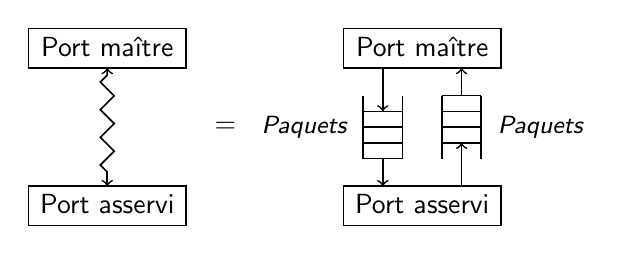
\begin{tikzpicture}
    \begin{scope}[shift={(0,0)}]
      \draw (0,2) rectangle node[text depth=0.3ex] {Port maître} ++(2,0.5);
      \draw (0,0) rectangle node[text depth=0.3ex] {Port asservi} ++(2,0.5);
      \queues{0}{0.5}
      \draw (2.5,1.25) node {=};
    \end{scope}

    \begin{scope}[shift={(4,0)}]
      \draw (0,2) rectangle node[text depth=0.3ex] {Port maître} ++(2,0.5);
      \draw (0,0) rectangle node[text depth=0.3ex] {Port asservi} ++(2,0.5);
      \queuesx{0}{0.5}
      \draw (-0.5,1.25) node {\small\it Paquets};
      \draw (2.5,1.25) node {\small\it Paquets};
    \end{scope}
  \end{tikzpicture}
\end{document}
